\documentclass[12pt,compress,aspectratio=169]{beamer}
\usetheme{metropolis}
\setbeamersize{text margin left=.5cm,text margin right=.5cm}
\usepackage[lf]{carlito}
\usepackage{siunitx}
\usepackage{tikz}
\usepackage{mathpazo}
\usepackage{bm}
\usepackage{mathtools}
\usepackage[ISO]{diffcoeff}
\diffdef{}{ op-symbol=\mathsf{d} }
\usepackage{xcolor,colortbl}


\title{Class 5: Center of Mass}
\subtitle{Advanced Placement Physics C}
\author[TML]{Dr.\ Timothy Leung}
\institute{Olympiads School}
\date{Updated: Summer 2022}

\newcommand{\pic}[2]{
  \includegraphics[width=#1\textwidth]{#2}
}
\newcommand{\eq}[2]{
  \vspace{#1}{\Large
    \begin{displaymath}
      #2
    \end{displaymath}
  }
}
%\newcommand{\iii}{\ensuremath\hat{\bm{\imath}}}
%\newcommand{\jjj}{\ensuremath\hat{\bm{\jmath}}}
%\newcommand{\kkk}{\ensuremath\hat{\bm{k}}}
%\newcommand{\iii}{\ensuremath\hat x}
%\newcommand{\jjj}{\ensuremath\hat y}
%\newcommand{\kkk}{\ensuremath\hat z}


\begin{document}

\begin{frame}
  \maketitle
\end{frame}



\begin{frame}{Center of Mass}
  Finding an object's center of mass is important, because
  \begin{itemize}
  \item The laws of motion are formulated by treating an objects as point
    masses (for real-life objects, we let the forces apply to the center of
    mass)
  \item Objects can have \emph{rotational} motion in addition to
    \emph{translational} motion as well (we will examine that a bit more in a
    very-important topic later)
  \end{itemize}
\end{frame}



\begin{frame}{Start with a Definition}
  The \textbf{center of mass} (``CM'') is the \emph{weighted average of the
    masses in a system.} The ``system'' may be:
  \begin{itemize}
  \item A collection of individual particles
  \item A continuous distribution of mass with constant density. In this case,
    CM is also the geometric center (\textbf{centroid}) of the object
  \item A continuous distribution of mass with varying density
  \item If the masses are inside of a gravitational field, then the CM is also
    its \textbf{center of gravity} (``CG'')
  \end{itemize}
\end{frame}



\begin{frame}{Simple Example}
  Start with a very simple example: two equal masses $m$ along the $x$-axis,
  located at $x_1$ and $x_1$. What is the center of mass of the system?
  \begin{center}
    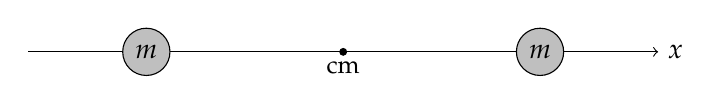
\begin{tikzpicture}
      \draw[->] (-4,0)--(4,0) node[right]{$x$};
      \draw[fill=lightgray] (-2.5,0) circle(.3) node{$m$};
      \draw[fill=lightgray] (2.5,0) circle(.3) node{$m$};
      \fill circle(.05) node[below]{\small cm};
    \end{tikzpicture}
  \end{center}
  The answer is simple: the half way point between them:

  \eq{-.1in}{
    x_\text{cm}=\frac{x_1+x_2}2
  }

  Multiply both numerator and denominator by mass $m$ (for generalization
  later), the equation becomes:

  \eq{-.1in}{
    x_\text{cm}=\frac{mx_1+mx_2}{2m}
  }
\end{frame}

 
\begin{frame}{Slightly More Challenging}
  What if one of the masses are increased to $2m$? This is still not a
  difficult problem; you can still \emph{guess} the right answer without
  knowing the equation for center of mass. 
  \begin{center}
    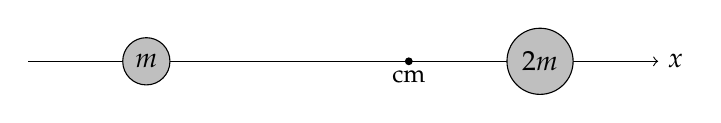
\begin{tikzpicture}
      \draw[->] (-4,0)--(4,0) node[right]{$x$};
      \draw[fill=lightgray] (-2.5,0) circle(.3) node{$m$};
      \draw[fill=lightgray] (2.5,0) circle(.42) node{$2m$};
      \fill(2.5/3,0) circle(.05) node[below]{\small cm};
    \end{tikzpicture}
  \end{center}
  The answer is still simple. The CM is no longer half way between the two
  masses, but now $\frac13$ the total distance from the larger masses. We can
  show using a weighted average:
  
  \eq{-.1in}{
    x_\text{cm}=\frac{mx_1+(2m)x_2}{m+2m}
  }  
\end{frame}



\begin{frame}{Complicating Things Further}{Many Point Masses}
  The weighted average concept can now be applied to cases when there are
  masses in 2D or 3D:
  \begin{center}
    \vspace{-.2in}
    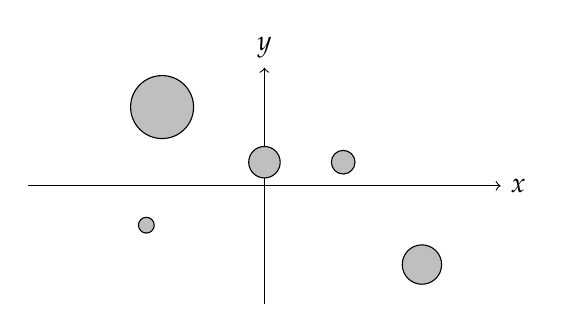
\begin{tikzpicture}
      \draw[->] (-3,0)--(3,0) node[right]{$x$};
      \draw[->] (0,-1.5)--(0,1.5) node[above]{$y$};
      \draw[fill=lightgray] (-1.3,1) circle(.4);
      \draw[fill=lightgray] (-1.5,-.5) circle(.1);
      \draw[fill=lightgray] (1,.3) circle(.15);
      \draw[fill=lightgray] (0,.3) circle(.2);
      \draw[fill=lightgray] (2,-1) circle(.25);
    \end{tikzpicture}
  \end{center}
\end{frame}



\begin{frame}{An Equation Helps}
  The center of mass is defined for discrete number of masses with the weighted
  average:

  \eq{-.1in}{
<<<<<<< HEAD
<<<<<<< HEAD
    \boxed{
      \vec x_\text{cm}=\frac{\sum \vec x_i m_i}{\sum m_i}
    }
=======
    \boxed{\vec x_\text{cm}=\frac{\sum \vec x_i m_i}{\sum m_i}}
>>>>>>> 2022-09-fall
=======
    \boxed{\vec x_\text{cm}=\frac{\sum \vec x_i m_i}{\sum m_i}}
>>>>>>> ce7a159 (Lots of commits!)
  }
  \begin{center}
    \begin{tabular}{l|c|c}
      \rowcolor{pink}
      \textbf{Quantity} & \textbf{Symbol} & \textbf{SI Unit} \\ \hline
      Position of center of mass (vector) & $\vec x_\text{cm}$ & \si\metre \\
      Position of point mass $i$ (vector) & $\vec x_i$ & \si\metre \\
      Point mass $i$ & $m_i$ & \si{\kilo\gram}
    \end{tabular}
  \end{center}
  In components:

  \eq{-.1in}{
    x_\text{cm}=\frac{\sum x_i m_i}{\sum m_i}\quad\quad
    y_\text{cm}=\frac{\sum y_i m_i}{\sum m_i}\quad\quad
    z_\text{cm}=\frac{\sum z_i m_i}{\sum m_i}
  }
\end{frame}



\begin{frame}{An Example}
  \textbf{Example:} Consider the following masses and their coordinates
  which make up a ``discrete mass'' rigid body''
  \begin{align*}
    m_1&=\SI{5.0}{\kg} &\vec x_1&=3\iii-2\kkk\\
    m_2&=\SI{10.0}{\kg}&\vec x_2&=-4\iii+2\jjj+7\kkk\\
    m_3&=\SI{1.0}{\kg}&\vec x_3&=10\iii-17\jjj+10\kkk
  \end{align*}
  What are the coordinates for the center of mass of this system?
\end{frame}



\begin{frame}{Continuous Mass Distribution}
  When the number of masses approaches infinity, this becomes a continuous
  distribution of mass. Taking the limit of masses $N\rightarrow\infty$ gives
  the integral form of our equation:

  \eq{-.1in}{
    \boxed{\vec x_\text{cm}=\frac{\int\vec x\dl m}{\int\dl m}}
  }

  What is the infinitesimal mass $\dl m$ then?
\end{frame}



\begin{frame}{Densities}
  Linear density (for 1D problems)

  \eq{-.1in}{
    \gamma = \diff mL\quad\rightarrow\quad \dl m =\gamma\dl L
  }

  Surface area density (for 2D problems)

  \eq{-.1in}{
    \sigma=\diff mA\quad\rightarrow\quad \dl m =\sigma\dl A
  }

  Volume density (for 3D problems)

  \eq{-.1in}{
    \rho=\diff mV\quad\rightarrow\quad \dl m =\rho\dl V
  }
  
  The densities do not have to be constant
\end{frame}


\begin{frame}{An Example with Integrals}
  \begin{columns}
    \column{.65\textwidth}
    \textbf{Example 2:} A triangular plate is placed in a Cartesian coordinate
    system with two of its edges along the $x$ and $y$-axis. The length of the
    edges along the axes are $a$ and $b$ respectively. Assuming that the
    surface area density $\sigma$ is uniform, determine the coordinate of its
    center of mass.

    \column{.35\textwidth}
    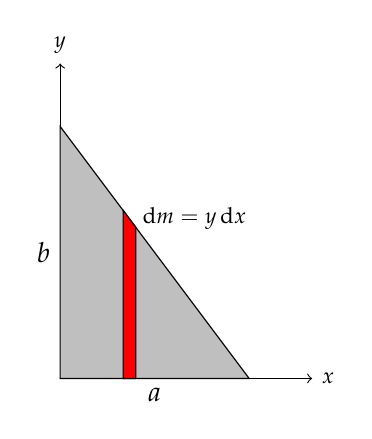
\begin{tikzpicture}[scale=.8]
      \draw[->](0,0)--(4,0) node[right]{\footnotesize $x$};
      \draw[->](0,0)--(0,5) node[above]{\footnotesize $y$};
      \draw[fill=lightgray](0,0)--(3,0) node[midway,below]{$a$}
      --(0,4)--cycle node[midway,left]{$b$};
      \uncover<2->{
        \draw[fill=red](1,0)--(1.2,0)--(1.2,2.4)--(1,2.67)
          node[midway,right]{\footnotesize $\dl m=y\dl x$}--cycle;
      }
    \end{tikzpicture}
  \end{columns}
\end{frame}



%\begin{frame}{A Difficult Example to Try at Home}
%  Not typically an AP problem, this example shows how we can use integral to
%  find the center of mass for something very complicated.
%  \begin{columns}
%    \column{.6\textwidth}
%    \textbf{Example 3:} Find the $x$-coordinate of the center of mass in the
%    shape bound by the two functions shown on the right.
%
%    \column{.4\textwidth}
%    \begin{tikzpicture}[scale=3]
%      \draw[->](0,0)--(1.25,0) node[right]{\footnotesize $x$};
%      \draw[->](0,0)--(0,1.25) node[above]{\footnotesize $y$};
%      \draw[fill=green!40]
%      plot[smooth,samples=40,domain=0:1] (\x,{\x*\x*\x})--
%      plot[smooth,samples=40,domain=1:0] (\x,{\x^(.5)});
%      
%      \draw[red!70,thick]  plot[smooth,samples=40,domain=0:1] (\x,{\x*\x*\x});
%      \draw[blue!70,thick] plot[smooth,samples=40,domain=0:1] (\x,{\x^(.5)});
%      \node at (.4,.85){\textcolor{blue!70}{\footnotesize $y=\sqrt{x}$}};
%      \node at (.9,.3){\textcolor{red!70}{\footnotesize $y=x^3$}};
%    \end{tikzpicture}
%  \end{columns}
%\end{frame}



\begin{frame}{Symmetry}{There are always shortcuts!}
  \begin{itemize}
  \item Any plane of symmetry, mirror line, axis of rotation, point of inversion
    \emph{must} contain the center of mass.
  \item Caveat: only works if the density distribution is also symmetric
  \item Again: if density is uniform, CM is also geometric center (centroid)
  \end{itemize}
\end{frame}



\begin{frame}{``Negative Mass''}{A Mathematical Trick}
  \begin{itemize}
  \item Where there is a ``hole'' in the geometry, treat it as having negative
    mass density $-\sigma$ in that region.
  \item Negative masses don't exist, so this is really just a trick.
  \item\textbf{Example:} What is the center of mass of this shape?
    \begin{center}
      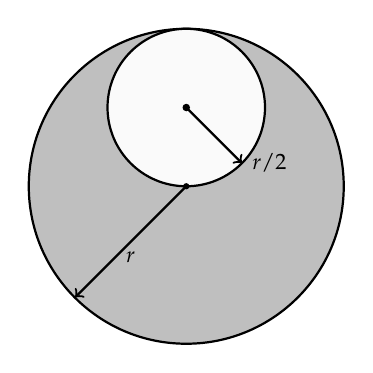
\begin{tikzpicture}
        \draw[thick,fill=lightgray] circle(2);
        \draw[thick,fill=black!2](0,1) circle(1);
        \fill circle(.04);
        \draw[thick,->](0,0)--(-1.41,-1.41)node[midway,below]{\footnotesize$r$};
        \draw[fill=black](0,1) circle(.04);
        \draw[thick,->](0,1)--(.707,.293) node[right]{\footnotesize$r/2$};
      \end{tikzpicture}
    \end{center}
  \end{itemize}
\end{frame}



\begin{frame}{Negative Mass Example}
  \begin{itemize}
  \item This is how we would think of it:
    \begin{center}
      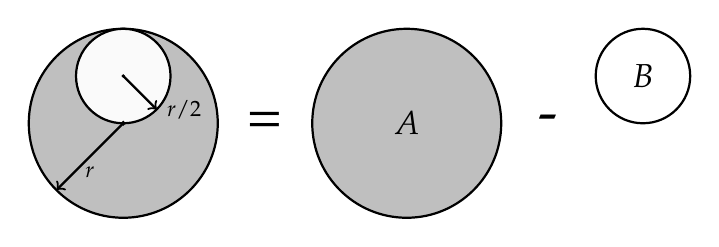
\begin{tikzpicture}[scale=.6]
        \draw[thick,fill=lightgray] circle(2);
        \draw[thick,fill=black!2](0,1) circle(1);
        \draw[fill=black](0,0) circle(.04);
        \draw[thick,->](0,0)--(-1.41,-1.41)
        node[midway,below]{\footnotesize$r$};
        \fill (0,1) circle(.04);
        \draw[thick,->](0,1)--(.707,.293) node[right]{\footnotesize$r/2$};
      
        \draw[thick,fill=lightgray](6,0) circle(2) node{\large$A$};
        \draw[thick](11,1) circle(1) node{\large$B$};
        \node at (3,0) {\huge=};
        \node at (9,0) {\huge -};
      \end{tikzpicture}
    \end{center}
  \item Let the origin of the coordinate system to located at the center of $A$
  \item Based on symmetry: $x_\text{cm}=0$; only have to find $y$-coordinate.
  \end{itemize}

  \eq{-.2in}{
    y_\text{cm}
    =\frac{\sum y_i m_i}{\sum m_i}
    =\frac{m_A(0) + m_B (r/2)}{m_A+m_B}
    =\frac{-\sigma\pi\left(r/2\right)^2(r/2)}
    {\sigma\pi r^2-\sigma\pi\left(r/2\right)^2}
    =\frac{-r}6
  }
\end{frame}



<<<<<<< HEAD
<<<<<<< HEAD
\begin{frame}{Velocity and Momentum}
  The time derivative of $\vec x_\text{cm}(t)$ is the velocity of the center of
  mass $\vec v_\text{cm}$:
    
  \eq{-.1in}{
    \vec v_\text{cm}=\diff{\vec x_{cm}}t
    =\frac1{m_\text{tot}}\diff{}t\left(\int\vec x\dl m\right)
    =\frac1{m_\text{tot}}\int\diff{\vec x}t\dl m
    =\frac{\int\vec v\dl m}{m_\text{tot}}
  }

  Rearranging the terms, we have:

  \eq{-.1in}{
    \int\vec v\dl m = m_\text{tot}\vec v_\text{cm}
  }

  The integral on the left hand side of the equation is the \textbf{net
    momentum} (i.e.\ the total of the momentum of all the masses). It is simply
  the momentum evluated using the velocity of the center of mass.
\end{frame}



\begin{frame}{Acceleration of the Center of Mass}
  
%  the system ($\vec p_\text{net}$) which means that we have
%
%  \eq{-.1in}{
%    \vec p_\text{net}=m\vec v_\text{cm}
%    }
  Taking the derivative of $\vec p_\text{net}$ relates force and acceleration
  at the CM as well:
    
  \eq{-.1in}{
    \vec F_\text{net}=\diff{\vec p_\text{net}}t=m\diff{\vec v_\text{cm}}t
    =m\vec a_\text{cm}
=======
%\begin{frame}{Velocity, Acceleration and Momentum}
%  Take time derivative of the equation for $\vec x_\text{cm}$ to get the
%  velocity at the CM:
%    

%  The integral in the numerator is the sum of the momentum of all the masses in
%  the system ($\vec p_\text{net}$) which means that we have
%
%  \eq{-.1in}{
%    \vec p_\text{net}=m\vec v_\text{cm}
%    }
%
%  Taking the derivative of $\vec p_\text{net}$ relates force and acceleration
%  at the CM as well:
%    
%  \eq{-.1in}{
%    \vec F_\text{net}=\diff{\vec p_\text{net}}t=m\diff{\vec v_\text{cm}}t
%    =m\vec a_\text{cm}
%  }
%\end{frame}



\begin{frame}{Velocity of the Center of Mass}
  Take time derivative of the equation for $\vec x_\text{cm}$ to get the
  velocity at the center of mass:

  \eq{-.1in}{
    \vec v_\text{cm}=\diff{\vec x_\text{cm}}t
    =\frac1m\diff{}t\left(\int\vec x\dl m\right)
    =\frac1m\int\diff{\vec x}t\dl m
    =\frac{\int\vec v\dl m}m
=======
%\begin{frame}{Velocity, Acceleration and Momentum}
%  Take time derivative of the equation for $\vec x_\text{cm}$ to get the
%  velocity at the CM:
%    

%  The integral in the numerator is the sum of the momentum of all the masses in
%  the system ($\vec p_\text{net}$) which means that we have
%
%  \eq{-.1in}{
%    \vec p_\text{net}=m\vec v_\text{cm}
%    }
%
%  Taking the derivative of $\vec p_\text{net}$ relates force and acceleration
%  at the CM as well:
%    
%  \eq{-.1in}{
%    \vec F_\text{net}=\diff{\vec p_\text{net}}t=m\diff{\vec v_\text{cm}}t
%    =m\vec a_\text{cm}
%  }
%\end{frame}



\begin{frame}{Velocity of the Center of Mass}
  Take time derivative of the equation for $\vec x_\text{cm}$ to get the
  velocity at the center of mass:

  \eq{-.1in}{
    \vec v_\text{cm}=\diff{\vec x_\text{cm}}t
    =\frac1m\diff{}t\left(\int\vec x\dl m\right)
    =\frac1m\int\diff{\vec x}t\dl m
    =\frac{\int\vec v\dl m}m
  }

  Or, in the form that is familiar, the velocity at the center of mass is the
  weighted sum of the velocities of the distribution of mass:
  
  \eq{-.1in}{
    \vec v_\text{cm} = \frac{\int\vec v\dl m}m
>>>>>>> ce7a159 (Lots of commits!)
  }

  Or, in the form that is familiar, the velocity at the center of mass is the
  weighted sum of the velocities of the distribution of mass:
  
  \eq{-.1in}{
    \vec v_\text{cm} = \frac{\int\vec v\dl m}m
>>>>>>> 2022-09-fall
  }

  The net force acting on the object is related to the acceleration of the
  center of mass
\end{frame}



\begin{frame}{Velocity and Momentum}
  We can also rearrange the equation for the velocity of the center of mass to
  relate it to momentum, because the term $\int\vec v\dl m$ is the net momentum
  of the mass distribution $p_\text{net}$:
  
  \eq{-.05in}{
    \vec v_\text{cm} = \frac{\int\vec v\dl m}m
    \quad\longrightarrow\quad
    \vec p_\text{net}=m\vec v_\text{cm}
  }

  During a collision, there is no change in the net momentum\footnote{Because
  there are are no external forces}, the center of mass will continue to move
  at the same velocity before/after the collision, as if the collision never
  occurred.
\end{frame}



\begin{frame}{Acceleration of the Center of Mass}
  Finding the rate of change of the net momentum (i.e\ applying the 2nd law of
  motion to this distribution of masses):
  
  \eq{-.1in}{
    \diff{\vec p_\text{net}}t =
    \diff{}t (m\vec v_\text{cm})
  }

  If the system mass is constant, then this equation reduces to:

  \eq{-.1in}{
    \diff{\vec p_\text{net}}t
    =m\diff{\vec v_\text{cm}}t
    \quad\longrightarrow\quad
    \boxed{
      \vec F_\text{net}=m\vec a_\text{cm}
    }
  }
  
  We can see that when a net force is applied to an object, the object's
  acceleration is evaluated at the center of mass.
\end{frame}



\begin{frame}{Velocity and Momentum}
  We can also rearrange the equation for the velocity of the center of mass to
  relate it to momentum, because the term $\int\vec v\dl m$ is the net momentum
  of the mass distribution $p_\text{net}$:
  
  \eq{-.05in}{
    \vec v_\text{cm} = \frac{\int\vec v\dl m}m
    \quad\longrightarrow\quad
    \vec p_\text{net}=m\vec v_\text{cm}
  }

  During a collision, there is no change in the net momentum\footnote{Because
  there are are no external forces}, the center of mass will continue to move
  at the same velocity before/after the collision, as if the collision never
  occurred.
\end{frame}



\begin{frame}{Acceleration of the Center of Mass}
  Finding the rate of change of the net momentum (i.e\ applying the 2nd law of
  motion to this distribution of masses):
  
  \eq{-.1in}{
    \diff{\vec p_\text{net}}t =
    \diff{}t (m\vec v_\text{cm})
  }

  If the system mass is constant, then this equation reduces to:

  \eq{-.1in}{
    \diff{\vec p_\text{net}}t
    =m\diff{\vec v_\text{cm}}t
    \quad\longrightarrow\quad
    \boxed{
      \vec F_\text{net}=m\vec a_\text{cm}
    }
  }
  
  We can see that when a net force is applied to an object, the object's
  acceleration is evaluated at the center of mass.
\end{frame}


%\begin{frame}{What This All Means}
%  \begin{itemize}
%  \item Newton was right all along by treating all objects as point masses
%    located at the CM
%  \end{itemize}
%\end{frame}

\end{document}
